\chapter{相關研究}
\label{章:相關研究}

\begin{figure}
\centerline{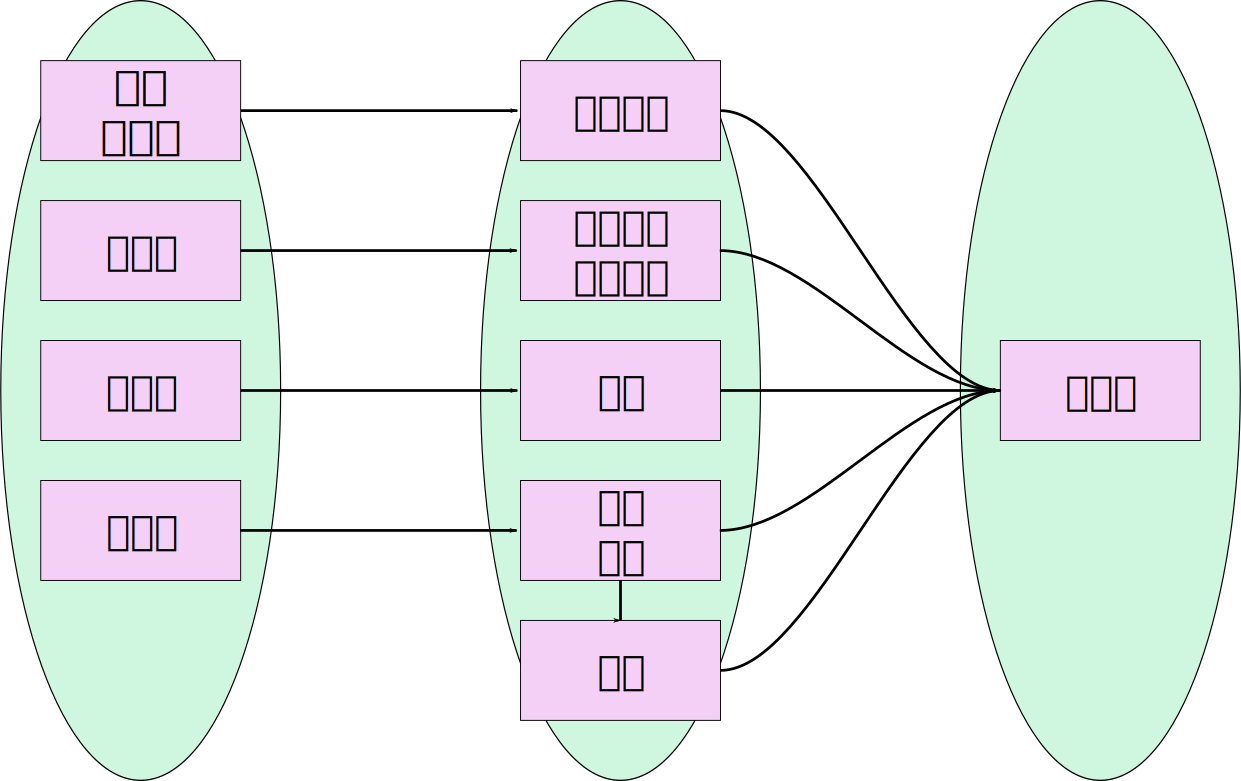
\includegraphics[keepaspectratio,width=40em]{圖/相關研究智識}}
\caption{逐門自然語言處理對應到相關的語言學}
\label{圖:相關研究智識}
\end{figure}

%漢語聲韻學→拼音系統
%語音學→語音合成、辨識
%音韻學→變調
%句法學→斷詞、剖析、翻譯
%語料庫

華語到閩南語的翻譯是自然語言處理(Natural Language Processing)\footnote{人講的話攏是自然語言}的一部份,
佇處理自然語言的時陣就需要語言相關的智識,會當簡單整理做圖\ref{圖:相關研究智識},
無仝的研究方向,愛知影的嘛無仝。
紲落來就介紹語言學佮自然語言處理的研究文獻佮母語的研究狀況。

\section{音標系統}
\label{節:音標系統}
音標系統有兩種,一種是研究語音用的記音系統,一種是予一般人拼寫用的拼音系統。

\subsection{記音系統}
\label{小節:記音系統}
研究一个語言,愛先了解伊的語音,
這時陣就需要一个標準化的記音符號。
這馬上時行的是國際語言學會(International Phonetic Association)制定的
國際音標(International Phonetic Alphabet,IPA)\cite{WIKI國際音標},
毋管記錄的語言有仝款無,只要語音的特徵仝款,就會用仝款的符號。

\subsection{拼音系統}
\label{小節:拼音系統}
記音的音標符號較濟,有的符號是較罕得看著,用起來無方便。
實際寫文章、編教材大部份會用另外的音標系統。
下跤照歷史年代簡單介紹閩南語主要三種拼音系統:

\subsubsection{臺灣閩南語羅馬字拼音}
臺灣閩南語羅馬字拼音是中華民國教育部佇2008年發佈的拼音方案,簡稱做臺羅。
伊的前身是教會羅馬字(白話字)\cite{WIKI教會羅馬字}
佮臺灣語言音標(Taiwan Language Phonetic Alphabet,TLPA)\cite{WIKI臺灣語言音標},
這馬猶原相容教會羅馬字。


\subsubsection{方音符號}
方音符號,又稱方言音符號\cite{華、台語注音符號溯源}
將華語的注音符號閣加一寡聲母、韻母佮聲調符號來標注閩南語。
是1946年朱兆祥教授設計,
佇1998年時,中華民國教育部嘛捌公告使用過。

\subsubsection{通用拼音}
余伯泉教授\ji{⿱毛灬}頭,想欲統一華語、閩南語、客語佮原住民語的拼音系統。
中華民國教育部佇2002年到2008年規定華語通用拼音當做譯音標準。

\subsubsection{音標比較表}
國際音標 臺羅 方音 通用 例字


\section{語音學}
\label{節:語音學}

\begin{table}
\caption{元音表}
\label{表:元音表}
\centering
\begin{tabular}{c|ccc}
\diaghead{\theadfont Diag ColumnmnHead II}{喙舌懸低}{喙舌前後}
%喙唇扁/圓 
& 頭前 & 中央 & 後壁\\
\hline
懸 & [i] & [ɨ] & [u]\\
中懸 & [e] &  & [o]\\
中 &  & [ə] & \\
中低 & [ɛ] &  & [ɔ]\\
低 & [a] &  & [ɑ]\\
\end{tabular}
\end{table}

\begin{table}
\caption{輔音表}
\label{表:輔音表}
\centering
\begin{tabular}{c|ccc}
\diaghead{\theadfont Diag ColumnmnHead II}{發音方式}{喙舌所在}
& 喙唇 & 中央 & 後壁\\
\hline
清塞音 & [i] & [ɨ] & [u]\\
濁塞音 & i & ɨ & u\\
鼻音 & [e] &  & [o]\\
邊音 &  & ə & \\
擦音 & ɛ &  & ɔ\\
\end{tabular}
\end{table}

語音學(Phonetics)主要討論喙舌的運動方式佮語音的物理性質。

前國際語言學會會長John Ohala捌講過:
「語音變化是連續的(Continuous),為著研究只好假設做離散特徵(Discrete)的音素(Phoneme)。」
可比講「\tsoo{狗}{⿳⿳ㄍㄠˋ}{kau2}」,
音標寫做[kau],
實際上[k]佮[a]、[a]佮[u]中央有誠濟過渡的音,
毋過過渡的音實在傷濟,
無法度一个一个寫出來,
只好用[k]、[a]佮[u]三个符號代表「\tsoo{狗}{⿳⿳ㄍㄠˋ}{kau2}」的音標。

語音會當用氣流有順無,
大略仔分做元音(Vowel)佮輔音(Consonant)。
表\ref{表:元音表}是幾仔个閩南語定用的元音,
會當看著[i]佮[u]攏是喙舌較懸發的音,
而且喙舌佇i發音時比u發音閣較頭前,
這嘛影響著\ji{⿰因}的頻譜(Frequency Spectrum),
[i]佮[u]共振鋒(Formant)嘛小可無仝。
[i]佮[u]喙型嘛無仝,
唸「\tsoo{ㄨ}{}{u}」的時陣喙尖尖,
唸「\tsoo{ー}{}{i}」的時陣喙較平,
嘛影響著語音的變化。
%裂 sai sai:伊笑甲~~~
%裂喙:伊笑的時陣攏會~~

若了解語音學,
就會當知影語音變化的道理,
支持音韻學的理論。

\section{音韻學}
\label{節:音韻學}
現代的音韻學(Phonology)是對Ferdinand de Saussure\cite{de2011course}提出語言學研究,
必須分做共時(Synchronic Linguistics)佮歷史(Diachronic Linguistics)兩種語言學。

共時語言學就是討論
音素是…
鼻音
討論變化,心中所想音檔→唸出來

歷史語言學
ian ien en

\section{漢語聲韻學}
\label{節:漢語聲韻學}
聲韻學是研究漢語自古到現代,方言的變化佮語音規律,
算是專門研究漢語的歷史語言學。

自三國南北朝時就有韻冊\footnote{李登《聲類》、呂靜《韻集》},
韻冊會記錄逐个字的反切,共仝韻母的字下做伙。
反切是古代中國用的記音方式,反切記音需要記兩个字,
一字代表聲母,一字代表韻母,
親像閩南語的「\tsoo{東}{⿳ㄉㄤ}{tang}」會用「\tsoo{端}{⿳ㄉ}{t}」「\tsoo{通}{⿳ㄤ}{ang}」表示。%用「車」?

到這馬上早上完整的文獻是宋國官修的廣韻\cite{2002廣韻注漳州漢音}\cite{2010新校互註宋本廣韻},
伊是綜合中國北方佮南方的語音系統。
嘛因為廣韻是綜合各地的系統,
伊記錄的反切嘛會當佇無仝的漢語方言用,
除了閩南語的「東」會當切做「端通」
華語的「\tsoo{東}{⿳⿳ㄉㄨㄥ}{}」嘛會當反切做「\tsoo{端}{⿳ㄉ}{}」「\tsoo{通}{⿳ㄨㄥ}{}」

嘛因為韻冊記錄是反切,毋是實際發音音值,
誠濟聲韻學家音韻學的理論,佮現代方言的材料,
來推測古早漢語的實際發音,
擬一套發音系統。

%狗頭後
%師詩斯


\section{句法學}
\label{節:句法學}
討論啥物是詞、詞的用法。句型

陸XX

\section{變調}
\label{節:變調}

準做想欲共臺語的字變做臺語的聲音,咱必須佮字,先標一對一斷詞,揣出音標。
但是臺語的變調是足複雜的,無法度予HTS內底的決策樹來做
所以愛先用另外一支程式專門來變調
楊允言教授就有做過\cite{iunn:台語變調系統實作研究},伊是用規則來確定變調的狀況,毋過伊用的語料無蓋濟,若數量一濟,規則式的變調會較歹處理。
變調嘛會當用機器學習的方法來做,共規則式用掉的特徵做伙下入去,看佗一个分類模型會較好,毋過伊上大的好處就是伊管理方便,免拄著啥物新語料,規則就愛全部重改,伊干焦需要共新語料加入重訓練就好矣,毋過伊的內部試驗就無保證一定著矣。

\section{語音辨識}
\label{節:語音辨識}
語音辨識就是共聲音轉做文字,會當用佇語音指令佮問答系統\footnote{親像蘋果公司的Siri}。
主流的做法是先共聲音轉做MFCC特徵
%\footnote{用MFCC特徵\cite{MFCC特徵}是因為實驗的效果上好\cite{MFCC上好}}
,
閣配合音檔的文本,
用隱性馬可夫模型\footnote{語音的變化當作狀態的轉移,而且聲音訊號是連續,無固定長度的特性。請看\ref{小節:隱性馬可夫模型}節。}
佮一个分類器\footnote{請看\ref{節:分類器}節}
訓練出辨識模型。

這方面的開源工具有HTK佮Kaldi:

\subsection{HTK}
\label{小節:HTK}
HTK全名號做Hidden Markov Model Toolkit\cite{HTK網頁},
發展的時間較早\footnote{對1989年到最近上新的2009年版本},
伊主要用\ref{小節:高斯混合模型}的高斯混合模型當做分類器。

HTK的模型訓練腳本\footnote{會當參考附錄\ref{章:臺灣言語工具}的臺灣言語工具,內底有提共HTK訓練佮使用的腳本},
一開始會先照文本的音,共音檔平均切做一个一个,
HTK流程圖~~

%決策樹
%wfst

\subsection{Kaldi}
\label{小節:Kaldi}
Kaldi\cite{Kaldi:Povey_ASRU2011}是較新的工具,
除了訓練一開始嘛是佮HTK仝款用高斯混合模型以外,
伊訓練後壁閣加入其他演算法,
效果比HTK閣較好。
%伊上大的特色是後壁分類器閣用深層類神經網路\cite{DNN},

%SGMM

\section{語音合成}
\label{節:語音合成}
語音合成是佮文字轉做聲音,佮語音辨識顛倒反,
親像車站廣播,有聲冊攏是語音合成的應用。
這馬時行的做法有兩種:

\subsection{模型合成}
\label{小節:模型合成}
這个方法頭一步是
先用人工抑是語音辨識軟體標記音檔的音,
共全部的音的特徵訓練出一个模型,
等欲合聲音時,才閣照模型的特徵,
用合成器合聲音出來。


\subsubsection{HTS}
\label{小節:HTS}
這方面開源軟體有HTS(HMM-based Speech Synthesis System)\cite{HTS網頁},
伊是對HTK修改來的。
用mgc、lf0、duration做聲音特徵,

伊訓練方式,
伊一个聲音會分做5个state\footnote{下跤講著的5狀態、三連音,攏是參數,毋是固定的},
逐个state有一个高斯模型,
伊會先訓練逐个音的初步模型,
閣來訓練三連音模型,
閣用決策樹共相倚的音綁做伙。

合的時陣才閣查決策樹,
共mgc、lf0、duration查出來,
閣用合成器合語音出來。

HTS只需要3000~7000句的訓練語料,
伊的輸出語音,
韻律攏袂\ji{⿰禾黑},
毋過因為聲音先轉做特徵,
特徵閣轉轉語音,
聲音的品質比原本的聲音會較\ji{⿰禾黑}一寡。

%伊需要音檔,標記發音內容的音檔,閣有音類的問題集。設計標仔。
%標仔的時間會使對HTK訓練。
%根據經驗,3000句會使,5000句普通,7000句上好。

\subsection{接聲音合成}
\label{小節:接聲音合成}

優點是聲音品質誠好,缺點是語料愛有夠濟,因為

\subsection{語音合成相關系統}
\label{小節:語音合成相關系統}
佇1999年林川傑就提出閩南語翻譯佮語音合成系統\cite{中文到閩南語之線上翻譯及閩南語之語音合成},

\section{斷詞}
\label{節:斷詞}
有一寡語言現象是佮詞有關係,
親像閩南語的變調,
毋過漢語語句的文本,
定定是一定一字無分開,
就看袂出來倒底佗一字佮佗一字是一个詞,
所以就需要斷詞,
共詞佮詞分開,
後壁的應用才有法度繼續落去。



華語這方面有中研院中文斷詞系統(CKIP)\cite{CKIP論文}。

閩南語斷詞的標準,
自誠早以前就有人討論矣\cite{台語斷詞原則討論},
教育部嘛有出「臺灣閩南語羅馬字拼音方案連字符使用原則」\cite{臺羅拼音},
定義連字符的標準。

%斷詞的標準有誠濟種,為著方便,以教育部的「臺灣閩南語羅馬字拼音方案連字符使用原則」的連字符當做一个詞,若「tsiah8 png7」(食白米飯的意思),當做兩个詞,「tsiah8-png7」(食物件的意思),當做一个詞。


%斷詞方法:長詞優先、配合語言模型、統計式、馬可夫、詞性

\subsection{長詞優先斷詞}
\label{節:長詞優先斷詞}

%定看著的斷詞方法有上長詞優先\footnote{(FMM)},伊的做法是自頭開始,看頭前幾个字是毋是會當揣著一个佇辭典的詞,若會使,就揀上長的彼个,…
%解釋比如說,『我想要吃飯』可以切成『我,想,要,吃,飯』『我,想要,吃飯』『我,想要吃飯』『我想要,吃飯』『我想要吃飯』,其中,能夠在字典找到詞的切割方式有『我,想,要,吃,飯』『我,想要,吃飯』,

\section{詞性標記}
\label{節:詞性標記}
\cite{iunn:利用統計方法及中文訓練資料處理台語文詞性標記}

\section{剖析}
\label{節:剖析}
斷詞了後毋知詞佮詞的關係
所以剖析
會當用佇翻譯佮語意分析(用佇問答系統)
楊允言教授有做過\cite{台語文語法結構樹建置}。
\section{翻譯}
\label{節:翻譯}
這馬電腦時行的翻譯方式是統計式機器翻譯(statistical machine translation),
這是對1993年Brown用數學證明\cite{brown1993mathematics}開始,
一直發展到這馬。
統計式機器翻譯會當分做對齊模型(alignment model)、語言模型(language model)佮解碼器(decoder)三个部份:

\subsection{對齊模型}
\label{小節:對齊模型}
對齊模型的功能是予解碼器知影詞愛按怎翻譯,
可比講是一个雙語的辭典。

對齊模型有分斷詞對齊佮剖析樹對齊兩種,下跤用斷詞對齊說明伊的原理。

先準備一組一組的華語閩南語平行語料,
親像「我 要 吃飯」和「我 欲 食 飯」,
紲落來產生語詞對照表。
華語詞的「要」,會對應到「我」、「欲」、「食」、「飯」閩南語詞,
經過大量的平行語料,
上尾知影華語的「要」定定對應著閩南語的「欲」,
也就是共對應頻率懸的組合留落來。
%改例

開源工具GIZA++\cite{och2003systematic}實作Brown 1993的演算法,
而且這馬嘛有支援多核心的MGIZA\cite{gao2008parallel}。

\subsection{語言模型}
\label{小節:語言模型}
第二部份是語言模型(language model),伊是欲用來判斷一句話是好是\ji{⿰禾黑}。

%加數學解釋
伊的做法是去記錄逐个詞後壁定定會接啥物詞,
若有一句話是「…欲 食…」,有「欲」佮「食」兩个詞,
咱知影「…欲 食」的後壁接「飯」比「…欲 食」的後壁接「湯」的機率較大,
也就是講「欲 食 飯」連紲詞比「欲 食 湯」連紲詞機率大,
若語言模型一擺看「欲 食 飯」三个詞,
就是三連紲詞模型(3-grams model)。
語言模型判斷一句話,伊出現的機率有偌大,就是看這句話伊內底連紲詞的機率是偌大。
%改例

這方面的工具有IRSTLM\cite{federico2008irstlm}、
SRILM\cite{stolcke2002srilm}佮
KenLM\cite{Heafield-estimate},
其中IRSTLM佮KenLM是LGPL開放授權,
SRILM是學術授權。

\subsection{解碼器}
\label{小節:解碼器}
上尾一部份是解碼器,
提面頂講的對齊模型、語言模型,
來翻譯華語到閩南語。

因為翻譯的問題毋是多項式時間(NP problem)會當解出來的,
所以解碼器袂使硬算全部的可能,
必須用有效率的演算法來翻譯。

上有名的開源程式就是Moses\cite{Koehn:2007:MOS:1557769.1557821},
伊整合對齊模型佮語言模型的介面,
閣有專工的訓練包通使用\cite{Moses訓練包}。

\subsection{評分方式}
\label{小節:評分方式}

翻譯大部份攏用BLEU(Bilingual Evaluation Understudy)來評分,
伊用連紲詞的概念來評分,
$BLEU=100\times{e^{\max{0,\frac{\textit{結果-答案長度}}{\textit{結果長度}}}}}\times{\sum_{n=1}^{4}(\textrm{n連紲詞})^{\frac{1}{4}}}$\cite{BLEU程式}。
%改cite

準若翻譯的答案是「這 幾 工 寒流 閣再 展威」,咱有兩个翻譯的結果,翻譯結果一「這 幾 工 寒流 有 展威」佮結果二「寒流 這 幾 工 閣再 展威」,請看表\ref{表:範例BLEU分數},答案有「這 幾 工」、「幾 工 寒流」、「工 寒流 閣再」佮「寒流 閣再 展威」4个三連紲詞,結果一有出現2个,所以結果一的三連紲詞分數是2/4,結果二有出現1个,分數是1/4。因為結果二無對應的四連紲詞,伊的分數都比結果一低。

\begin{table}
\caption{翻譯結果一「這 幾 工 寒流 有 展威」佮翻譯結果二「寒流 這 幾 工 閣再 展威」對答案「這 幾 工 寒流 閣再 展威」的分數}%
\label{表:範例BLEU分數}
\centering
\begin{tabular}{|c|cccc|c|}
\hline
翻著的數量 & 一連紲詞 & 兩連紲詞 & 三連紲詞 & 四連紲詞 & BLEU分數\\
\hline
結果一 & 5/6 & 3/5 & 2/4 & 1/3 & 53.73\\
\hline
結果二 & 6/6 & 3/5 & 1/4 & 0/4 & 0.00\\
\hline
\end{tabular}
\end{table}


\section{語料庫}
\label{節:語料庫}
自然語言處理需要語料才有法度訓練模型,
就需要語料庫共語料存起來。

\begin{table}
\caption{自然語言處理技術需要的語料庫}
\label{表:自然語言處理技術需要的語料庫}
\centering
\begin{tabular}{lc}
技術 & 語料樣式 \\
變調 & 原始文本、本調音標佮變調音標 \\
語音辨識 & 濟人音檔佮對應文本 \\
語音合成 & 孤人音檔佮對應文本 \\
斷詞 & 斷詞的語料 \\
剖析 & 剖析樹 \\
翻譯 & 兩種語言的平行語料 \\
\end{tabular}
\end{table}

有的語料庫是純文字的資料庫,
嘛有存音檔的語料庫,
愛看需求,定看著的技術會當參考表\ref{表:自然語言處理技術需要的語料庫}。

\subsection{閩南語語料種類}
\label{節:閩南語語料種類}

\begin{table}
\caption{閩南語語料種類比較表}
\label{表:閩南語語料種類比較表}
\centering
\begin{tabular}{lcc}
種類 & 範例 & 備註\\
全漢 & 我欲食飯 & 全部漢字\\
全羅 & gua2 beh4 tsiah8-png7 & 全部羅馬拼音,有斷詞資訊\\
漢羅 &我beh4食飯 & 漢字拼音濫咧用\\
\end{tabular}
\end{table}

閩南語是漢語的一支方言,
大部份的字攏會當揣著漢字,
毋過閩南語嘛毋是純漢語,
有的字無對應的漢字。

有的人慣勢全部用羅馬拼音創作,
這種寫法號做「全羅」。
嘛有人慣勢全部用漢字創作,
號做「全漢」
毋過有的字無法度揣著對應的漢字,
全漢實際上的拄著造字、揣字的困難,
為著創作方便,
知影的字用漢字寫,
賰的用音標寫落來,
號做「漢羅」。
詳細會當看表\ref{表:閩南語語料種類比較表}的範例。

\subsection{閩南語語料-新聞語料庫}
\label{節:新聞語料庫}
華語閩南語雙語語料庫\footnote{\url{http://icorpus.iis.sinica.edu.tw/}}(後壁用「新聞語料庫」稱呼)是何澤政\footnote{一九七零年代出世,臺中烏日人}對民國九十七年十一月初六開始,逐工揣兩篇華語新聞,先斷句,後尾翻譯做閩南語教會全羅。親像原本的新聞「這幾天寒流再度發威」,翻譯做「tsit4-kui2-kang han5-liu5 koh-tsai3 tian2-ui」(這幾工寒流閣再展威)\footnote{原文是教會羅馬字,為著文章一致,以教育部的臺羅書寫}。
新聞語料庫的翻譯罕得改變用詞的先後,親像面頂的「這幾天寒流再度發威」,較袂翻做「寒流這幾工閣再展威」,除非照華語用詞先後翻譯的結果無順,才會調整。

澤政佇語料內底用
「挕捒 hinn3-sak4」\footnote{挕捒意思共物件擲掉、放捒,嘛就是華話的「丟棄」,例句甲(家己做的):這支筆好好,為啥物愛共伊挕捒。例句乙(Tek-hôa,Nah ē teh批判民進黨?,\url{http://taioan-chouhap.myweb.hinet.net/089.htm}):民進黨接續李登輝的路線, 繼續加強黨國時代權力者, 倚附者佮既得利益者的優勢,毋是共刜挕捒。}
、
「作孽」\footnote{
青-少-年|tshing1-siau3-lian5 作-孽|tsok4-giat8 跤-踏-車|kha1-tah8-tshia1 擲|tan3 落|loh8 河-中|ho5-tiong1。

愛耍手賤,華語的「惡作劇」。例句甲:叫你莫摸你閣摸,誠實手賤愛作孽!(家己做的)例句乙:你這个作孽囡仔,你是按怎沐甲一身軀烏趖趖?(惠光,天真瀾漫,\url{http://ip194097.ntcu.edu.tw/nmtl/DADWT/thak.asp?id=992})}
本土的詞以外,伊嘛會配合這馬發生的代誌,用較時行的閩南語,親像
「喙罨」\footnote{華語的「口罩」}、
「心肌梗窒」\footnote{心|sim1 肌|ki1 梗|king2 窒|that4,華語的「心肌梗塞」}、
「自來水」\footnote{閩南語較古典的用法,會號做「水道水」}、…。
而且除了現代閩南語,澤政伊閣會去查台華線頂辭典\footnote{\url{http://ip194097.ntcu.edu.tw/iug/Ungian/SoannTeng/chil/Taihoa.asp}}
選擇較古典的用詞\footnote{台華線頂辭典是古早語料,一个詞若台華線頂辭典查有,教育部辭典查無,就當做伊是較古典的詞},親像
「𤺪|sian7 篤-篤|tauh4-tauh4」\footnote{熱-天|juah8-thinn1 高-溫|ko1-un1 炎-熱|iam7-juah8 規-工|kui1-kang1 𤺪|sian7 篤-篤|tauh4-tauh4 。|。}、「鬥-贊-手|tau3-tsan3-tshiu2」\footnote{佇|ti7 三|sam1 一-一|it4-it4 大-地-動|tua7-te7-tang7 慷-慨|khong2-khai3 鬥-贊-手|tau3-tsan3-tshiu2 ,|,}。

拄著外來詞,澤政嘛會選擇保留原文,拄著華語的「歐巴馬」佮「西藏」,會翻轉去英文「Obama」、「Tibet」。

斷詞組

加漢字,

若源頭是日本話外來詞,就會直接用教羅寫出來,請看

\subsection{閩南語語料-教育部辭典}
\label{節:教育部辭典}
這章按算加入教育部辭典佮數位典藏兩个語料庫,教育部辭典全名「臺灣閩南語常用詞辭典」\footnote{\url{http://twblg.dict.edu.tw/holodict_new/}},正式版是100年上線,伊有25892的詞條\footnote{1021230申請到的版本},內底誠濟生活的用語,大部份詞條攏有漢字、音標、解釋、佮例句。的翻譯。
嘛因為伊有漢字佮音標,就會當共遮的漢字佮音標收集起來,當做用字參考的字典,
這个辭典是教育部編的,當然漢字有照教育部家己的規範\footnote{臺灣閩南語推薦用字700字表,佇96~99年公佈修正}來寫,所以伊內部的用字前後有一致,為著翻譯的效果佮使用者的方便,就共教育部辭典的用字當做標準,若有用字佮教育部的用字無仝的,就改做教育部的用字。//閣愛順過

伊的例句,除了閩南語漢字佮音標以外,閣有敆華語的翻譯,親像表\ref{表:教育部辭典例句},漢字佮音標的對應會使提去做用字參考的字典,音標的部份會當提來斷詞,訓練語言模型,閩南語佮華語的對應會使提來做平行語料。這例句的語料是非常完整,攏總有8XXX句。
\begin{table}
\caption{教育部辭典例句}
\label{表:教育部辭典例句}
\centering
\begin{tabular}{l}
彼个查某囡仔真媠。 \\
Hit ê tsa-bóo gín-á tsin suí.\\
那個女孩子很漂亮。\\
\end{tabular}
\end{table}

除了一般的詞條以外,教育部辭典嘛有收一寡俗語、臆謎猜,攏做388句做附錄句。
因為附錄句干焦提供解釋,所以無法度提來做平行語料,毋過會使提來訓練語言模型。

台語文數位典藏資料庫\footnote{\url{http://xdcm.nmtl.gov.tw/dadwt/pbk.asp}}(下跤號做數位典藏)是國家臺灣文學館收集1885~2006年的語料,攏總2167篇。
照時代分做清國時期170篇、日治時代490篇,民國統治1507篇。內底嘛有照語料形式分做四類,有詩387條、散文1127篇、小說387篇、劇本49篇。攏總416343句。

因為伊是百外冬的語料庫,較古早的語料,用詞就較古典, %//閣再加

\subsection{閩南語語料-數位典藏}
\label{節:數位典藏}
數位典藏的來源語料百百款,臺文館⿰因為著格式統一,就替原底是全漢抑是漢羅的語料補全羅拼音\footnote{有時陣劇本邊仔的解釋會用漢字,親像「(福哥仔出場)」},若原本是全羅,就請人拍漢羅,會當看表\ref{表:數位典藏語料},拍漢羅的時,⿰因若知影漢字,就會拍漢字,賰的外來語,抑是較本土的語詞就會用音標來拍。
伊有的語料是一句對齊一句,有的是一段對齊一段。

\begin{table}
\caption{數位典藏語料漢羅、全羅對照}
\label{表:數位典藏語料}
\centering
\begin{tabular}{l}
漢羅:Koh m7知u7危險.........., \\
全羅:Koh m7-tsai u7 gui5-hiam2..............., \footnote{數位典藏內底原本是白話字(教會羅馬拼會),為著讀者方便,攏改做教育部的臺羅}\\
\end{tabular}
\end{table}


\subsection{閩南語語料-TGB通訊臺灣組合}
\label{節:TGB通訊-臺灣組合}
TGB通訊\footnote{\url{http://taioan-chouhap.myweb.hinet.net/}}是學生台灣語文促進會對1999年10月開始\footnote{\url{http://taioanchouhap.pixnet.net/blog/post/32374696}}一個月一期的刊物。頭前60期以閩南語為主,61期有提供華語對照,有時陣閩南語句內底會濫一寡華語詞,形式較無固定

因為有閩南語、有華語佮臺華平行語料,嘛閣有濫做伙的, 誠濟種實際會拄著的情形會當提來做判斷語言的語料。
有的時陣閩南語佮華語濫做伙,先定義啥物情形算閩南語,啥物情形算華語

用人工分

主要語句是閩南語,有一兩个詞是華語嘛是算閩南語
閩南語

聽人講 khah 早有出現過『小蜜蜂』
我 beh tńg 來種作 ! ── 記 0312 Truku 反亞泥 ‧ 還我土地運動
有台灣味 ê 繪本──《我和我的腳踏車》 .

華語
華語閩南語攏通的算華語
有華語完整的一句話就算華語
毋是華語嘛毋是閩南語,親像英文、日語、…

「 糟了 ,是工地火燒厝, 緊轉去打 火 ! 」建設公司 的 工地主任 從手機接到消息,通話結束後就帶著那群混混先離開了。
『聽說妳最近遇到什麼問題 , 是不是 ? 怎麼了 ? 』好性地 ê QA 繼續問--落-去 .
去越南胡志明市 4 工/越南胡志明市四日行 @Gio̍k-hōng

\subsection{閩南語語料腔口統計佮處理}
\label{小節:閩南語語料腔口統計佮處理}

\section{語料收集整理}
\label{節:語料收集整理}
佇這个網路的時代,收集語料上緊的方法就是去網路面頂掠。看圖XX,先共閩南語專門的字詞擲去搜尋引擊\footnote{親像Google、Bing},閣照揣著的網頁去掠相關的閩南語。
閩南語的網頁內底除了閩南語以外,有可能閣濫一部份的華語,為著莫予華語語料影響著閩南語模型,所以愛想辦法共臺華兩種語言分開。分開了後

%圖:關鍵詞 引擊 網址 掠網頁 網頁html 轉文字 一句一句的語料 判斷語言 閩南語/華語 對齊

\begin{figure}
\centerline{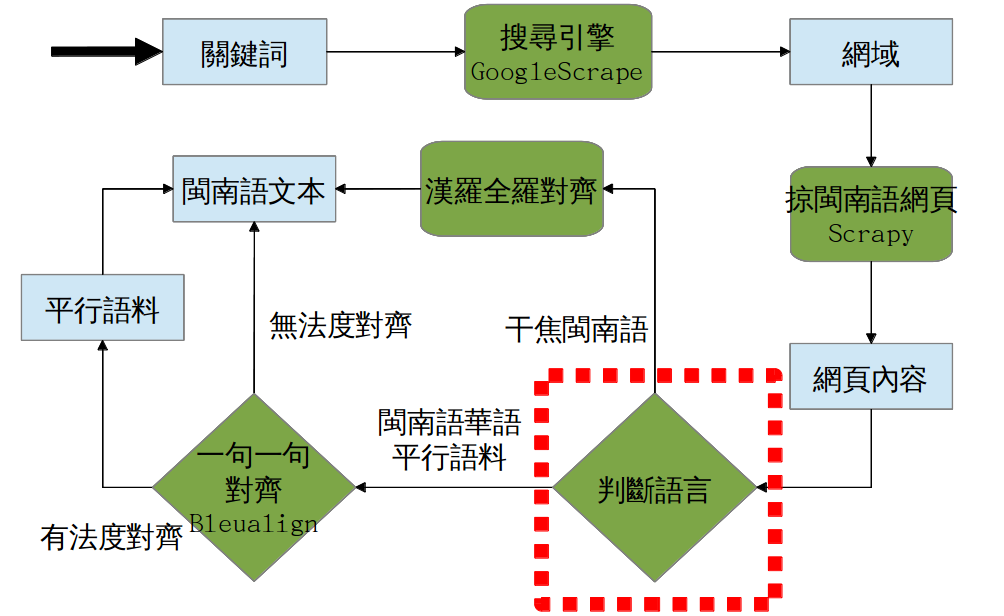
\includegraphics[keepaspectratio]{圖/網路語料庫結構}}
\caption{網路語料庫}
\label{圖:網路語料庫結構}
\end{figure}

\subsection{收集網路資料}
\label{小節:收集網路資料}

\subsection{語言分類}
\label{小節:語言分類}
南島語主要嘛是拼音文字,
所以會使用這个方法,
南島語佮漢語的語言分類較簡單,
就算漢語用羅馬拼音,
拼音的種類嘛差誠濟,
只要檢驗有聲調抑是拼音規則就會使判斷是南島語抑是漢語。


\subsection{語料對齊}
\label{小節:語料對齊}
bleualign


\section{分類器}
\label{節:分類器}

\subsection{隱性馬可夫模型}
\label{小節:隱性馬可夫模型}
隱性馬可夫模型(Hidden Markov Model,HMM)
%\cite{HMM}

\subsection{支持向量機}
\label{小節:支持向量機}

\subsection{決策樹}
\label{小節:決策樹}

\subsection{高斯混合模型}
\label{小節:高斯混合模型}


